\documentclass[journal]{IEEEtran}

\usepackage{amsmath}
\usepackage{amssymb}
\usepackage{bm}
\usepackage{booktabs}
\usepackage{subcaption}
\usepackage{hyperref}
\usepackage{svg}

\newcommand{\bx}{\bm{x}}
\newcommand{\by}{\bm{y}}
\newcommand{\bz}{\bm{z}}
\newcommand{\btheta}{\bm{\theta}}
\newcommand{\bphi}{\bm{\phi}}

\DeclareMathOperator{\expectation}{\mathbb{E}}

\begin{document}

\title{Adversarial Error Correction}

\author{Mayank Mishra (2016EE30506), Tarun Kumar Yadav (2016CS10359), Chahat Chawla (2016MT10492)}

\maketitle

\begin{abstract}
Deep neural networks have been enormously successful across a variety of classification tasks. However, recent research shows that DNNs are vulnerable to adversarial attacks, which pose a serious threat. In this paper, we propose a simple yet effective defense algorithm Adversarial Error Correction that uses variational autoencoder (VAE) to filter out adversarial noise from input images to a classifier. The proposed method is generic and can defend white-box attacks without the need of retraining the original CNN classifiers, and can further strengthen the defense.
\end{abstract}

\section{Introduction}
Deep neural networks are highly expressive models that have recently achieved
state of the art performance on speech and visual recognition tasks. Despite their ability to learn complicated functions, little is known about what they learn. Deep neural networks learn input-output mappings that are fairly discontinuous to a significant extent. We can cause the network to misclassify an image by applying a certain hardly perceptible perturbation, which is found by maximizing the network’s prediction error. In addition, the specific nature of these perturbations is not a random artifact of learning: the same perturbation can cause a different network, that was trained on a different subset of the dataset, to misclassify the same input.

Machine learning models are vulnerable to these small perturbations. Such examples with these perturbations are calles adversarial examples. These adversarial examples look similar to their non-adversarial counterparts but lead to poor classification accuracy of deep learning systems on a particular task.

\section{Adversarial attacks}
\subsection{Fast Gradient Sign Method (FGSM)}
FGSM\cite{FGSM} is a single step attack. Let $L(\bx, \by)$ be the loss function of the classifier C given input $\bx$ and target label $\by$. FGSM defines the perturbation $\bm{\rho}$ as
\begin{equation}
	\bm{\rho} = \epsilon \times sign(\nabla_{\bx} L(\bx, \by))
\end{equation}
where $\epsilon$ is a small factor. FGSM simply chooses the sign of change at each pixel to increase the loss $L(\bx, \by)$ and fool the classifier.

\subsection{Projected Gradient Descent}
PGD\cite{PGD} is a more powerful multi-step attack with projected gradient descent. Projected gradient descent performs one step of standard gradient descent, and then clips all the coordinates to be within the box for box-constrained numerical optimization. 
\begin{equation}
	\begin{aligned}
		& \bx_0^{PGD} = \bx
		\\
		\bx_{t+1}^{PGD} = \prod_S [\bx_t^{PGD} & + \alpha \times sign(\nabla_{\bx} L(\bx_t^{PGD}, \by))]
	\end{aligned}
\end{equation}
where $\prod_S$ is the projection onto $S = \{\bx' : ||\bx' - \bx||_{\infty} \leq \epsilon\}$.

\section{Variational Autoencoders}
Generative models have gained a lot of success since the advent of deep neural networks. In particular, GANs\cite{GAN} and VAEs\cite{VAE} have been used to model highly complex distributions whose implicit expressions might be intractable. We can obtain a lower bound on the log likelihood of the data as
\begin{equation}
	\log p(\bx) \geq -KL[q_{\bphi}(\bz | \bx) || p_{\btheta}(\bz)] + \expectation_{q_{\bphi}(\bz | \bx)}[\log p_{\btheta}(\bx | \bz)]
\end{equation}

To achieve the goal of maximizing the log-likelihood, one can simply maximize a lower bound, evidence lower bound (ELBO) on the log-likelihood. This can be done by using a VAE.

\section{Adversarial error correction}
We leverage the expressive capability of VAEs for defense mechanism. Our proposed method is generic and can defend white-box and black-box attacks and no online iterative optimisation is involved.

We modify the VAE objective (that preserves the adversarial perturbations in reconstruction) to the one which constructs the corresponding clean image, enabling to correctly label the adversarial image.

An adversarial example is passed through a VAE whose encoder is K-Lipschitz. From a coding theory perspective, we claim that latent representation codes for the adversarial and clean image will be closed in latent space when the encoder is K-Lipschitz. 

\begin{equation}
    \begin{aligned}
        \bz \sim & \operatorname{Enc}(\hat{\bx})=q(\bz | \hat{\bx})
        \\
        \bx \sim & \operatorname{Dec}(\bz)=p(\bx | \bz)
        \\
        \mathcal{L}= & -\expectation_{q(\bz | \hat{\bx})}\left[\log \frac{p(\bx | \bz) p(\bz)}{q(\bz | \hat{\bx})}\right]
        \\
        = & -\expectation_{q(\boldsymbol{z} | \hat{\bx})}[\log p(\bx | \bz)] + KL(q(\bz | \hat{\bx}) || p(\bz))
    \end{aligned}
\end{equation}

where $\hat{\bx} = \bx + \boldsymbol{\delta}$ is an adversarial image with $\delta$-perturbation added on top of a clean image $\bx$. This adversarial
image is encoded to a latent variable $\bz$, which is decoded
to the underlying clean image $\bx$.

\section{Experiments and results}
\subsection{Datasets}
For the purpose of this paper, we experimented on the Fashion MNIST dataset (black and white images of the dimension $28 \times 28$) and the SVHN dataset (coloured images of the dimension $32 \times 32$). Both datasets have 10 ground truth classes.

\subsection{Adversarial attacks}
We perform the two mentioned adversarial attacks in this paper i.e FGSM\cite{FGSM} and PGD\cite{PGD}. The resulting images generated using FGSM for Fashion MNIST are shown in Fig. \ref{fig:FMNISTFGSM}. The resulting images generated using PGD for Fashion MNIST are shown in Fig. \ref{fig:FMNISTPGD} and for SVHN in Fig. \ref{fig:SVHNPGD}.

\subsection{Defense mechanisms}
We try out two defense mechanisms to protect our classifiers as discussed below:

\subsubsection{Adversarial retraining}
We do adversarial retraining of the classifiers. Basically, in this approach the classifier are retrained on the adversarial examples.

\subsubsection{Adversarial error correction}
An adversarial example is passed through a VAE whose encoder is K-Lipschitz. From a coding theory perspective, we claim that latent representation codes for the adversarial and clean image will be closed in latent space when the encoder is K-Lipschitz. We experiment with both gradient norm penalty and gradient clipping for imposing Lipschitz constraint on encoder, and found the former to be giving slightly better results experimentally. Results in the table are reported with gradient norm penalty.

Our method can also be used as a simple detection mechanism to detect if an input image contains adversarial perturbations or not. This can be done by comparing the MSE between reconstructed image and the original image. If an image does contain adversarial perturbation, then this MSE measure will be relatively large as compared to when the image doesn’t contain adversarial perturbations (refer Fig. \ref{fig:distance}). Assuming perfect VAE, the exact added $\delta$-perturbation must be recovered after reconstruction. We set a criteria on this difference to detect the adversarial example, and results for the same has been reported in the table.

In this approach the adversarial examples are passed through a VAE whose encoder is K-Lipschitz. The claim is that if the encoder is K-Lipschitz the adversarial examples and the real examples would be close enough in the latent space. This Lipshitz contraint on the encoder is imposed by having a gradient penalty on the encoder.

\subsection{Further studies}
It is further seen that as the dimensionality of the latent space is increased the adversarial examples and the real data come closer in the latent space. (See Fig. \ref{fig:distance})

\begin{table*}[t]
	\caption{Accuracy on Fashion MNIST with and without defense mechanisms}
	\centering
	\begin{tabular}{c|c|ccc|c}
		\toprule
		& & \multicolumn{3}{c|}{Adversarial retraining} & Adversarial error correction
		\\
		\midrule
		Attack & No defense & FGSM 0.3 & PGD 0.1 & PGD 0.3 & VAE
		\\
		\midrule
		No attack & 91.2 & 91.4 & 89.9 & 91 & 82.2
		\\
		FGSM ($\epsilon = 0.1$) & 24.2 & 82.6 & 81 & 75.9 & 62.7
		\\
		FGSM ($\epsilon = 0.3$) & 9.1 & 89.4 & 42.4 & 74.4 & 49.2
		\\
		PGD ($\epsilon = 0.1$) & 5.9 & 12.1 & 71.7 & 61.8 & 50.5
		\\
		PGD ($\epsilon = 0.3$) & 5.7 & 5.6 & 7.1 & 68.1 & 44.2
		\\
		\bottomrule
	\end{tabular}
	\label{tab: cnnconv}
\end{table*}

\begin{table*}[t]
	\caption{Accuracy on SVHN with and without defense mechanisms}
	\centering
	\begin{tabular}{c|c|c}
		\toprule
		& & Adversarial error correction
		\\
		\midrule
		Attack & No defense & VAE
		\\
		\midrule
		No attack & 93.7 & 83.4
		\\
		FGSM ($\epsilon = 0.05$) & 11.4 & 66.4
		\\
		FGSM ($\epsilon = 0.1$) & 10.8 & 47.7
		\\
		PGD ($\epsilon = 0.05$) & 3.4 & 71.5
		\\
		PGD ($\epsilon = 0.1$) & 2.9 & 60.9
		\\
		\bottomrule
	\end{tabular}
	\label{tab: cnnconv}
\end{table*}

\begin{figure*}[t]
	\centering

	\begin{subfigure}{\textwidth}
		\centering
		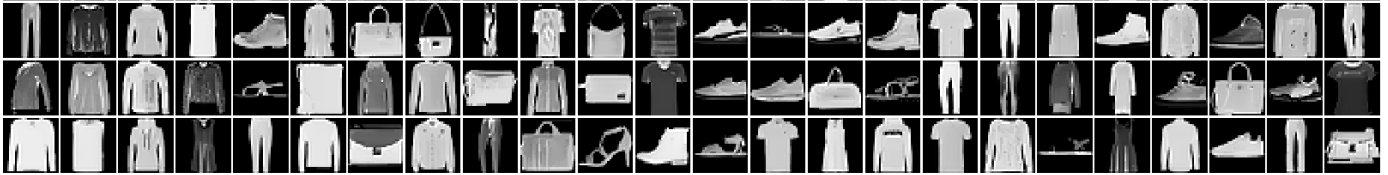
\includegraphics[width=\textwidth]{Images/MNIST/FGSM/Original.png}
		\subcaption{Original images}
	\end{subfigure}
	% \wspace{2mm}
	\begin{subfigure}{\textwidth}
		\centering
		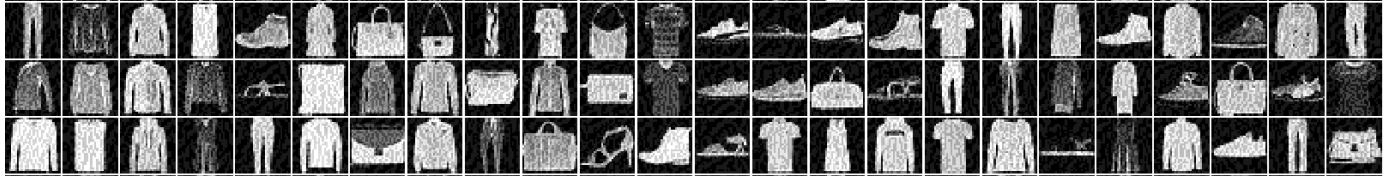
\includegraphics[width=\textwidth]{Images/MNIST/FGSM/FGSM.png}
		\subcaption{FGSM with $\epsilon = 0.3$}
	\end{subfigure}

	\caption{Fashion MNIST dataset comparing original and adversarial examples generated using FGSM\cite{FGSM} attack}
	
	\label{fig:FMNISTFGSM}
\end{figure*}

\section{Conclusion}
In this paper, we have proposed a simple yet effective defense algorithm Adversarial Error Correction that uses a variational autoencoder (VAE) to filter out adversarial noise from input images to a classifier. The proposed method is generic and can defend white-box and black-box attacks without the need of retraining the original classifiers, and can further strengthen the defense.

\bibliographystyle{ieeetr}
\bibliography{references}

\begin{figure*}[t]
	\centering

	\begin{subfigure}{\textwidth}
		\centering
		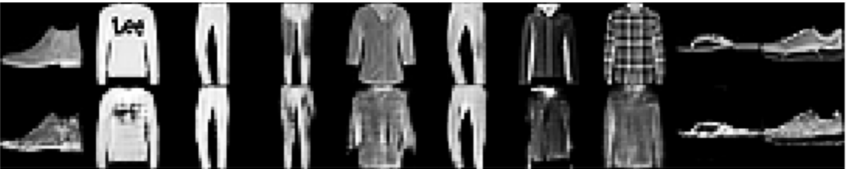
\includegraphics[width=\textwidth]{Images/MNIST/PGD/Original.png}
		\subcaption{Original images}
	\end{subfigure}
	% \wspace{2mm}
	\begin{subfigure}{\textwidth}
		\centering
		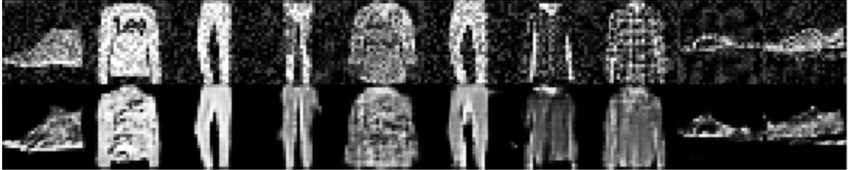
\includegraphics[width=\textwidth]{Images/MNIST/PGD/PGD.png}
		\subcaption{PGD with $\epsilon = 0.3$}
	\end{subfigure}

	\caption{Fashion MNIST dataset comparing original and adversarial examples generated using PGD\cite{PGD} attack}

	\label{fig:FMNISTPGD}
\end{figure*}

\begin{figure*}[t]
	\centering

	\begin{subfigure}{\textwidth}
		\centering
		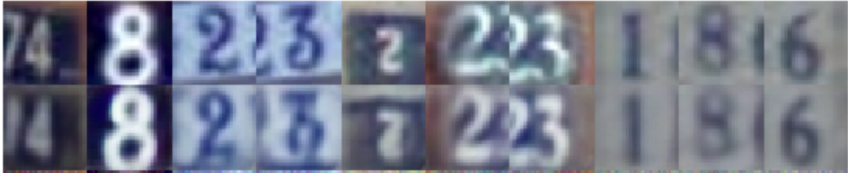
\includegraphics[width=\textwidth]{Images/SVHN/Original.png}
		\subcaption{Original images}
	\end{subfigure}
	% \wspace{2mm}
	\begin{subfigure}{\textwidth}
		\centering
		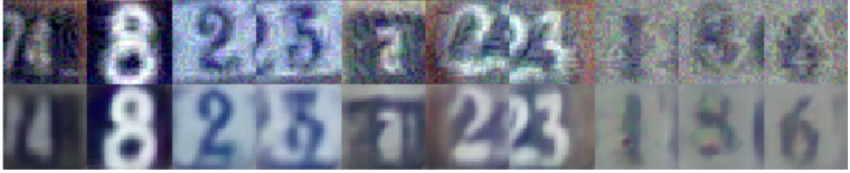
\includegraphics[width=\textwidth]{Images/SVHN/PGD.png}
		\subcaption{PGD with $\epsilon = 0.3$}
	\end{subfigure}

	\caption{SVHN dataset comparing original and adversarial examples generated using PGD\cite{PGD} attack}
	
	\label{fig:SVHNPGD}
\end{figure*}

\begin{figure*}[t]
	\centering
	\captionsetup{justification=centering}

	\begin{subfigure}{\textwidth}
		\centering
		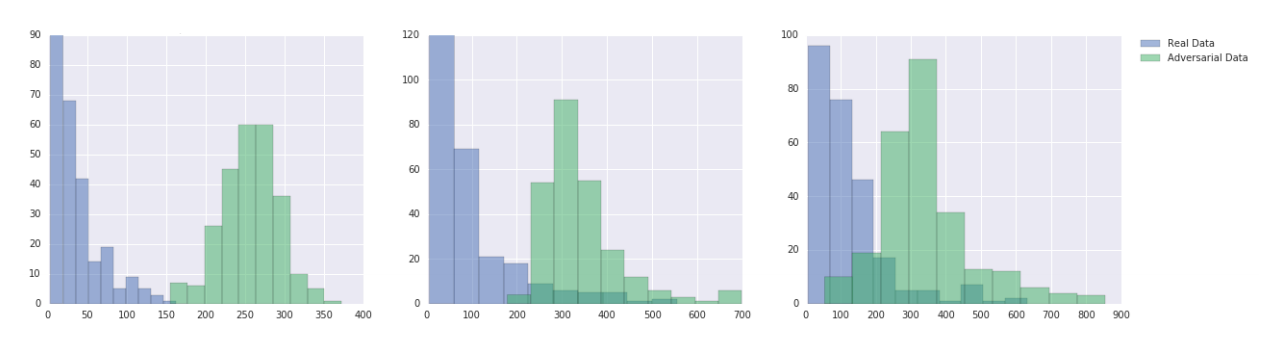
\includegraphics[width=\textwidth]{Images/VAE/MNIST.png}
		\subcaption{Fashion MNIST}
	\end{subfigure}
	% \wspace{2mm}
	\begin{subfigure}{\textwidth}
		\centering
		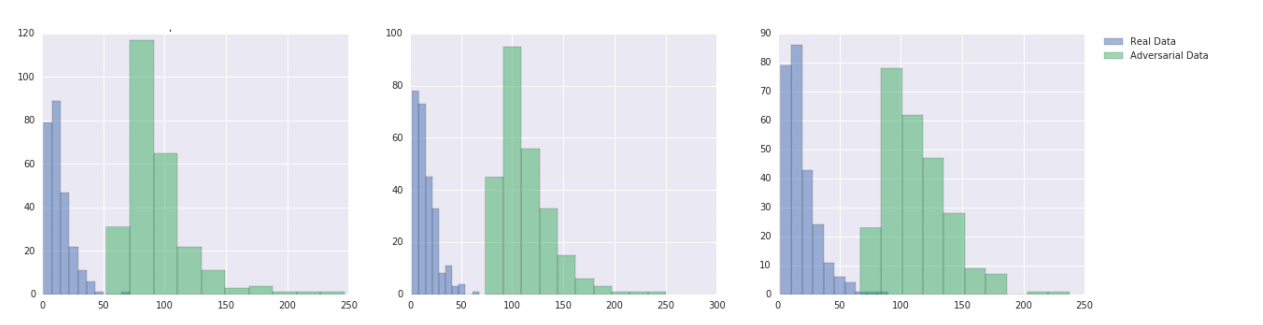
\includegraphics[width=\textwidth]{Images/VAE/SVHN.png}
		\subcaption{SVHN}
	\end{subfigure}

	\caption{x-axis is the $L_2$ norm of the real and adversarial latent spaces and y-axis is the number of samples. Clearly, the peaks come closer as the latent dimesionality increased. Latent dimensionality increases from left to right (32, 64, 128).}
	
	\label{fig:distance}
\end{figure*}

\end{document}